\section{Bài tập}\label{sec_3}

\textbf{Bài 1}: Sử dụng lại phương trình Poisson bên trên. Khảo sát các phương pháp số bằng cách thay đổi số nút và số phần tử của lưới để tìm ra ảnh hưởng của chúng đến độ chính xác. Ứng với mỗi phương pháp, xác định số nút và số phần tử tối uu để đạt được độ chính xác mong muốn. Vẽ đồ thị thể hiện sự phụ thuộc của sai số vào số nút và số phần tử.

\textbf{Bài 2}: Giải phương trình sau bằng các phương pháp số đã trình bày
\begin{equation}
    \begin{aligned}
        \frac{\partial^2 u}{\partial x^2} + u &= 0 \quad x \in \left(0, 1\right) \\
        u\left(0\right) &= 1 \quad \left(\hbox{điều kiện biên Dirichlet}\right) \\
    \end{aligned}
\end{equation}

\textbf{Bài 3}: Hệ dao động 6 bậc tự do
Hình dưới là một mô hình tối giản của một ô tô. Hệ này có 6 bậc tư do như trên hình. Mục đích của bài tập này là mô phỏng chuyển động của các bộ phận khi ô tô chuyển động và gặp một vật cản trên đường \cref{fig_6dofs}.

\begin{figure}[htbp]
    \centering
    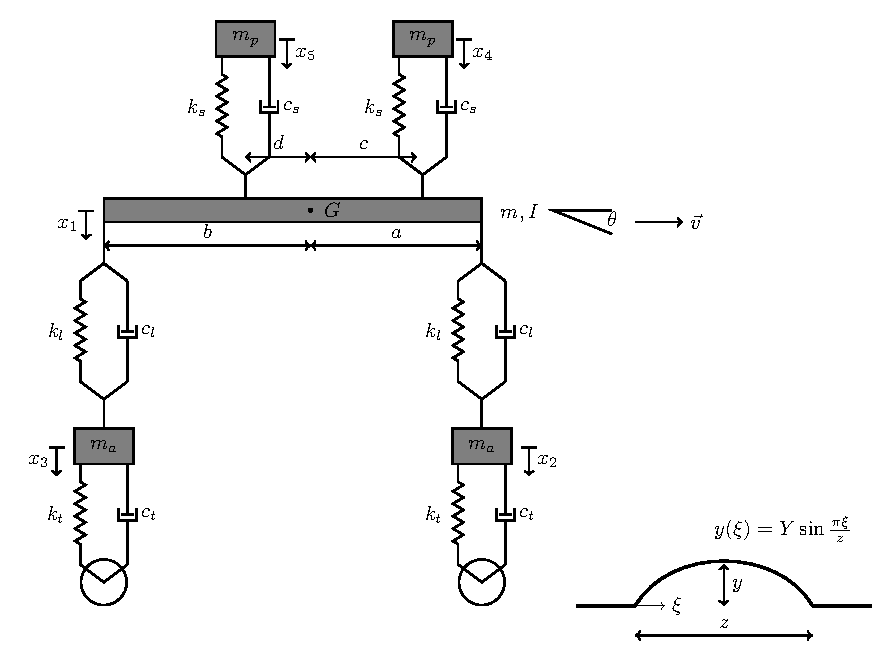
\includegraphics[width=1.\textwidth]{Tuan6/figure/6dofs.pdf}
    \caption{Hệ dao động 6 bậc tự do}
    \label{fig_6dofs}
\end{figure}

Cho các giá trị sau:
\begin{equation*}
    \begin{matrix}
        m = \SI{1000}{\kilogram} & k_l = \SI{120000}{\newton\per\meter} & a = \SI{1.8}{\meter} \\
        m_a = \SI{150}{\kilogram} & k_t = \SI{80000}{\newton\per\meter} &  b = \SI{2.0}{\meter} \\
        m_p = \SI{60}{\kilogram} & k_s = \SI{200000}{\newton\per\meter} &  c = \SI{0.6}{\meter} \\
        I = \SI{360}{\kilogram.\m^2} & v = \SI{40}{\meter\per\second} &  d = \SI{0.4}{\meter} \\
    \end{matrix}
\end{equation*}

Vector bậc tự do được biễu diễn như sau: ${\bf u} = \begin{bmatrix}
    \theta & x_1 & x_2 & x_3 & x_4 & x_5 \end{bmatrix}^T$

a) Chứng minh rằng ma trận độ cứng, ma trận giảm chấn và ma trận khối lượng của hệ dao động này có dạng:

\begin{equation}
    {\bf K} = \begin{bmatrix}
        \left(a^2+b^2\right) k_l+\left(c^2+d^2\right) k_s & (a-b) k_l+(c-d) k_s & -a k_l & b k_l & -c k_s & d k_s \\
        (a-b) k_l+(c-d) k_s & 2\left(k_l+k_s\right) & -k_l & -k_l & -k_s & -k_s \\
        -a k_l & -k_l & k_l+k_t & 0 & 0 & 0 \\
        b k_l & -k_l & 0 & k_l+k_t & 0 & 0 \\
        -c k_s & -k_s & 0 & 0 & -c k_s & 0 \\
        d k_s & -k_s & 0 & 0 & 0 & -k_s
    \end{bmatrix}
\end{equation}

\begin{equation}
    {\bf C} = \begin{bmatrix}
        \left(a^2+b^2\right) c_l+\left(c^2+d^2\right) c_s & (a-b) c_l+(c-d) c_s & -a c_l & b c_l & -c c_s & d c_s \\
        (a-b) c_l+(c-d) c_s & 2\left(c_l+c_s\right) & -c_l & -c_l & -c_s & -c_s \\
        -a c_l & -c_l & c_l+c_t & 0 & 0 & 0 \\
        b c_l & -c_l & 0 & c_l+c_t & 0 & 0 \\
        -c c_s & -c_s & 0 & 0 & -c c_s & 0 \\
        d c_s & -c_s & 0 & 0 & 0 & -c_s
    \end{bmatrix}
\end{equation}

\begin{equation}
    {\bf M} =\begin{bmatrix}
        I & 0 & 0 & 0 & 0 & 0 \\
        0 & m & 0 & 0 & 0 & 0 \\
        0 & 0 & m_a & 0 & 0 & 0 \\
        0 & 0 & 0 & m_a & 0 & 0 \\
        0 & 0 & 0 & 0 & m_p & 0 \\
        0 & 0 & 0 & 0 & 0 & m_p
    \end{bmatrix}
\end{equation}

b) Xác định các mode dao động riêng của hệ. Tính tần số dao động riêng của hệ.

c) Áp dụng phương pháp tích phân số để mô tả chuyển động của hệ. Chúng ta lấy giá trị của ma trận giảm chấn ${\bf C} = \alpha{\bf M} + \beta{\bf K}$ với $\alpha = 0$ và $\beta = 5*10^{-4}$.